\documentclass[16pt, a4paper]{article}
\usepackage[utf8]{inputenc}
\usepackage[a4paper, total={6in, 8in}, margin = 1.5in]{geometry}
\usepackage{graphicx}
\graphicspath{{images/}}
\usepackage{amssymb}
\title{AI1110 Assignment 1}
\author{Hema Sri Cheekatla, CS21BTECH11013}
\begin{document}
\maketitle
ISCE 10 2018
\section*{Question 4a}
Solve the following inequation, write down the solution set and represent it on the real number line:

\[  -2 + 10x \leq 13x + 10 < 24 + 10x,  x\in \mathbb{Z} \]

\section*{Solution}
\[  -2 + 10x \leq 13x + 10 < 24 + 10x,  x\in \mathbb{Z} \]

Let us solve the above expression geometrically.

now consider each equation in this expression as a line equation

$y_1 = 10x - 2$

$y_2 = 13x + 10$

$y_3 = 10x + 24$

clearly slopes of $y_1$ and $y_3$ are same i.e., $slope = 10$\newline
and $y_1 \leq y_2 < y_3 $, so the integral values of x on x-axis satisfying this inequality are the required solution set\newline
so we need to find the range of x at where the line $y_2$ lies between between line $y_1$ and the line $y_3$

We can obtain the x value at intersection point of $y_1$ and $y_2$ by equating them that is,


$\hspace{16pt}\hspace{16pt} y_1 = y_2$

$\Rightarrow 10x - 2 = 13x + 10$

$\Rightarrow -10 -2 = 13x - 10x$

$\Rightarrow -12 = 3x$

$\Rightarrow x = -4$

Similary we get the x value at intersection point of $y_2$ and $y_3$ by equating $y_2$ and $y_3$


$\hspace{16pt}\hspace{16pt} y_3 = y_2$

$\Rightarrow 10x + 24 = 13x + 10$

$\Rightarrow 24 - 10 = 13x - 10x$

$\Rightarrow 14 = 3x$

$\Rightarrow x = 4.67$


Since $y_1 \leq y_2 < y_3$, this implies $-4 \leq x < 4.67$


Now let us draw the corresponding lines

\begin{figure}[h]
    \centering
    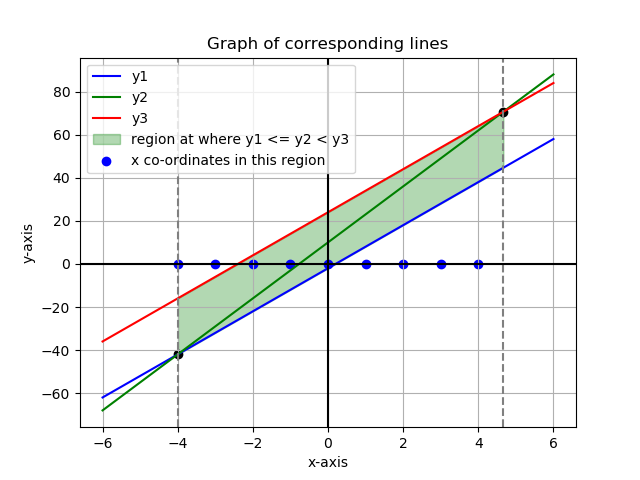
\includegraphics[width = 0.75\textwidth]{Figure_1}
    \caption{lines $y_1$, $y_2$ and $y_3$}
    \label{fig:mesh1}
\end{figure}

If we observe this graph, it is clear that the lines $y_1$ and $y_2$ are intersecting at $x = -4$ and the lines $y_2$ and $y_3$ are intersecting at some point where $x>4$

Hence the required range of x is $[\-4, 4.67)\ $\newline


\vspace{16pt}
Therefore the integers in this range are,

\begin{center}
\begin{tabular}{|c|}
\hline
\textbf{$ \{ -4, -3, -2, -1, 0, 1, 2, 3, 4\}$} \\
\hline
\end{tabular}
\end{center}


here is the plot of corresponding points on the real number line\\
\begin{figure}[h]
    \centering
    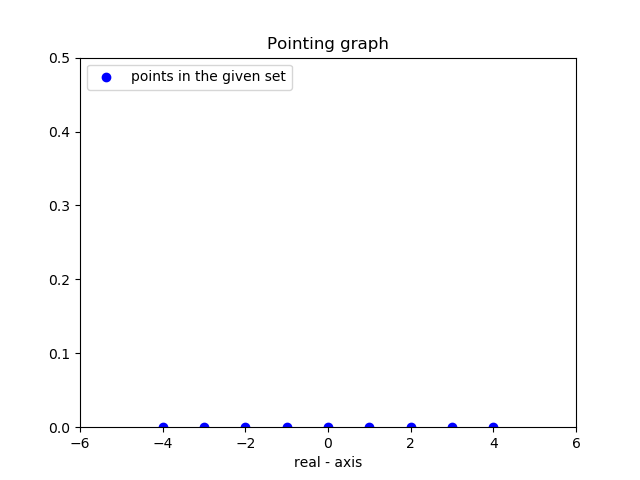
\includegraphics[width = 0.5\textwidth]{Figure_2}
    \caption{set of points that obey given expression on real number line}
    \label{fig:mesh1}
\end{figure}
\end{document}
